\chapter{Σχετική Εργασία και Θεωρία στην Αρχιτεκτονική} 
\label{chap:Literature}

\section{Σχετική Εργασία}

Τα τελευταία χρόνια γίνεται μια προσπάθεια να τυποποιηθούν τα 
peer-to-peer συστήματα σε μια ενιαία αρχιτεκτονική. Πιο γενικά σε ένα 
μοντέλο αναφοράς όπου περιγράφονται βασικές οντότητες και 
αλληλεπιδράσεις και βάσει αυτού μπορούν να κατασκευαστούν τέτοια 
συστήματα.

Στην δημοσίευση \citep{F.Dabek2003} έχουμε τον διαχωρισμό του συστήματος 
σε τρία επίπεδα. Το πρώτο επίπεδο αφορά την δρομολόγηση η οποία βασίζεται σε κλειδιά 
(key-based routing). Πάνω σε αυτό χτίζονται τα πρωτόκολλα του συστήματος 
\begin{wrapfigure}{l}{0.5\textwidth}
  \begin{center}
    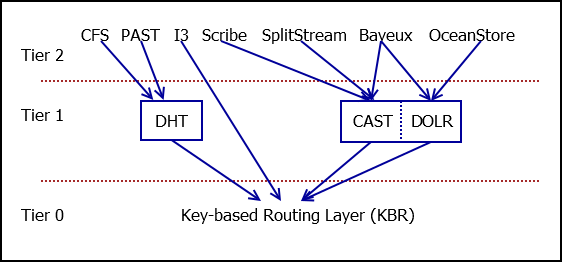
\includegraphics[width=0.48\textwidth]{Figures/Related_work/Towards_a_common_API_(tiers).png}
  \end{center}
  \caption{Towards a common API}
  \label{fig:Α_common_API}
\end{wrapfigure}
όπως κατανεμημένοι πίνακες κατακερματισμού (DHT), αποκεντρωμένη 
τοποθεσία αντικειμένου και δρομολόγησης (Decentralized Object Location 
and Routing) καθώς και anycast/multicast λειτουργικότητα. Οι εφαρμογές 
έχουν πρόσβαση που αποτελούν το ανώτερο αρχιτεκτονικό επίπεδο, έχουν 
πρόσβαση απευθείας στα δυο κατώτερα επίπεδα. Οι διεπαφές που 
προτείνονται όμως δεν μπορούν να καλύψουν όλες τις ανάγκες. Στο σχήμα  
\ref{fig:Α_common_API} φαίνονται τα επίπεδα της προτεινόμενης αρχιτεκτονικής.

Ο εμπνευστής του PGrid συστήματος με την ομάδα του εισάγει ένα 
μοντέλο αναφοράς \citep{Aberer05theessence} στο οποίο μπορούν να σχεδιαστούν 
διάφορα peer-to-peer συστήματα. Στο σχήμα \ref{fig:Essence} παρουσιάζονται τα 
αρχιτεκτονικά επίπεδα του μοντέλου. Στηρίζεται πάνω στο επίπεδο του 
δικτύου το οποίο συγκεντρώνει τα πρωτόκολλα   
\begin{wrapfigure}{l}{0.45\textwidth}
  \begin{center}
    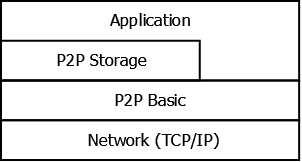
\includegraphics[width=0.43\textwidth]{Figures/Related_work/The_essence_of_p2p_(architecture).png}
  \end{center}
  \caption{Προτεινόμενη αρχιτεκτονική από Aberer et al.}
  \label{fig:Essence}
\end{wrapfigure}
TCP/IP. Αυτό παρέχει τις λειτουργίες του στο βασικό επίπεδο (P2P basic) το οποίο και υλοποιεί το 
peer-to-peer δίκτυο. Οι λειτουργίες που παρέχει είναι η σύνδεση (join) 
και η αποχώρηση (leave) στο δίκτυο, αναζήτησης (lookup) και δρομολόγησης 
(route). Στη συνέχεια έχουμε το επίπεδο αποθήκευσης (P2P storage) που 
παρέχει λειτουργίες εισαγωγής (insert), διαγραφής (delete), ανανέωσης 
(update) δεδομένων στο δίκτυο καθώς και τη διενέργεια ερωτήσεων πάνω σε 
αυτά (query). Για την ανάπτυξη μιας εφαρμογή, χρησιμοποιούνται οι 
διεπαφές που προσφέρονται από το βασικό επίπεδο και αυτό της 
αποθήκευσης. Στο σχήμα \ref{fig:Essence_UML} παρουσιάζεται το 
προτεινόμενο βασικό μοντέλο.

\begin{figure}[htbp]
  \begin{center}
    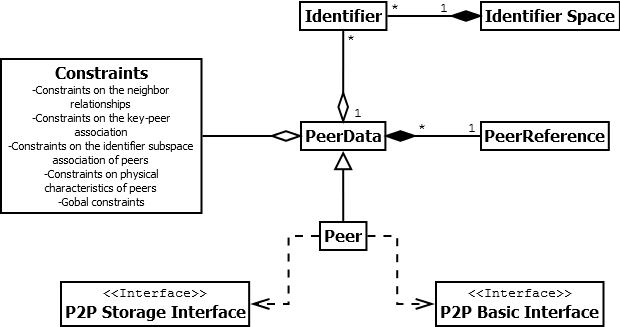
\includegraphics[scale=0.55]{Figures/Related_work/The_essence_of_p2p_(uml).png}
  \end{center}
  \caption{Προτεινόμενο μοντέλο αναφοράς από Aberer et al.}
  \label{fig:Essence_UML}
\end{figure}

Σε αυτό φαίνονται τα απαραίτητα συστατικά που προκύπτουν από την 
ανάλυση, οι διάφοροι περιορισμοί που τίθενται και οι διεπαφές που πρέπει 
να υποστηρίζει κάθε peer-to-peer σύστημα. Στην υλοποίηση του PGrid από 
τον Schmidt \citep{Schmidt2007}, ακολουθήθηκε το παραπάνω 
μοντέλο. Η όλη λογική είναι ένα peer-to-peer σύστημα να είναι χαλαρά 
συνδεδεμένο με τις υπηρεσίες που προσφέρουν το βασικό επίπεδο και αυτό 
της αποθήκευσης. Στόχος είναι η ευκολία αλλαγής συμπεριφοράς του ίδιου 
συστήματος εναλλάσσοντας τις διάφορες υλοποιήσεις. Παρόλα αυτά όπως 
προκύπτει από την εξέταση της υλοποίησης, είναι δύσκολο να επεκταθεί μια 
υπάρχουσα υλοποίηση με άλλα πρωτόκολλα πιο πολύπλοκα.

\begin{wrapfigure}{L}{0.5\textwidth}
  \begin{center}
    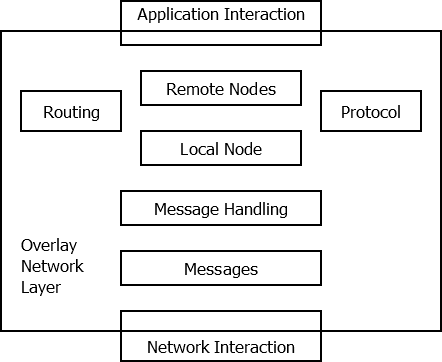
\includegraphics[width=0.48\textwidth]{Figures/Related_work/A_pattern_language.png}
  \end{center}
  \caption{A Pattern Language}
  \label{fig:Patterns}
\end{wrapfigure}

Για την εσωτερική δομή επιπέδων όπως αυτό του βασικού της παραπάνω 
αρχιτεκτονικής , έχουμε μια προσπάθεια να δημιουργηθούν σχεδιαστικά 
πρότυπα. Στις δημοσιεύσεις \citep{Grolimund2005, Grolimund2006} αναλύονται 
ένα σύνολο peer-to-peer συστημάτων και ενδιάμεσου λογισμικού. Από αυτό 
προκύπτουν σχεδιαστικά πρότυπα που έχουν να κάνουν με ένα βασικό στοιχείο 
αυτών των συστημάτων που είναι η δρομολόγηση των μηνυμάτων μέσα στο δίκτυο. 
Στο σχήμα \ref{fig:Patterns} φαίνεται η αρχιτεκτονική δομή του συγκεκριμένου επιπέδου. 
Κάθε στοιχείο του επιπέδου περιλαμβάνει μια σειρά σχεδιαστικών προτύπων. 

Στη δημοσίευση \citep{Amoretti2005} εισάγεται η έννοια 
του Peer ως σχεδιαστικό πρότυπο. Το πρόβλημα που προσπαθεί να επιλυθεί 
είναι η αποτελεσματική κατανομή του φόρτου εργασίας και η υψηλή 
διαθεσιμότητα των πόρων. Η λογική είναι παρόμοια μόνο που πλέον οι πόροι 
και οι λειτουργίες που προσφέρει ένας peer παρουσιάζονται ως υπηρεσίες. 
Ενδιαφέρει ο τρόπος με τον οποίο περιγράφονται οι υπηρεσίες και 
προτείνεται η ύπαρξη είτε μιας WSDL διεπαφής όπου μπορεί να ανακτηθεί 
πλήρως η λειτουργικότητα της είτε OWL-S περιγραφών σε περίπτωση που 
είναι αναγκαία η σημασιολογική περιγραφή (semantic) της πληροφορίας. 
Προτείνεται, μάλιστα, η χρήση Web Service αρχιτεκτονικής δεδομένου των 
πλεονεκτημάτων που μπορεί να φέρει μια τέτοια υπηρεσία. 

Από την πρακτική εφαρμογή του προτύπου \citep{Amoretti2005SP2A}. 
Χρησιμοποιήθηκαν τεχνολογίες όπως η JXTA και Web Services. Για την ανάπτυξη 
των τελευταίων χρησιμοποιήθηκαν τα JXTA-SOAP και OWL-S. Η περιγραφή των web 
service μέσω OWL-S κάνει εύκολη την ανακάλυψη, την εκτέλεση, την σύνθεση 
αυτών και την παρακολούθηση τους (monitoring). Παρόλα αυτά, το συγκεκριμένο 
framework υποστηρίζει υβριδικά και καθαρά peer-to-peer δίκτυα χωρίς όμως να 
υπάρχει συγκεκριμένη τοπολογία. Επίσης, δεν υπάρχει η έννοια της 
σύνθεσης των υπηρεσιών στο ίδιο το λογισμικό του peer σε πιο πολύπλοκες 
διαδικασίες/πρωτόκολλα.

Σημαντική δουλειά είναι τα JXTA πρωτόκολλα \citep{JXTA2007}. Αυτά 
αποτελούν μια ανοιχτή διαδικτυακή πλατφόρμα για peer-to-peer συστήματα. 
Τυποποιείται ο τρόπος με τον οποίο ένας peer ανακαλύπτει άλλους, πώς 
οργανώνεται σε ομάδες peer και πως επικοινωνεί. Επίσης, ορίζονται 
πρωτόκολλα για την διαφήμιση και ανακάλυψη διαδικτυακών πόρων. Υπάρχουν 
τρία αρχιτεκτονικά επίπεδα με πρώτο το επίπεδο της πλατφόρμας όπου 
ορίζονται κλασικοί τύποι για ένα peer-to-peer δίκτυο. Στη συνέχεια 
έχουμε το επίπεδο των υπηρεσιών το οποίο περιλαμβάνει διαδικτυακές 
υπηρεσίες όπως αναζήτησης και ευρετηριοποίησης, αποθηκευτικού χώρου, 
διαμοιρασμού αρχείων, κατανεμημένα συστήματα αρχείων και άλλα. Το τελικό 
επίπεδο είναι αυτό της εφαρμογής που εκμεταλλεύεται τις προσφερόμενες 
υπηρεσίες. Δεν υπάρχει όμως καθορισμός της τοπολογίας των peer-to-peer 
δικτύων που προκύπτουν και τα πρωτόκολλα είναι ορισμένα ως ένα σύνολο 
από XML μηνύματα προκειμένου την ανεξαρτητοποίηση από λειτουργικά 
συστήματα και γλώσσες προγραμματισμού.

\section[Υπηρεσιοκεντρική Αρχιτεκτονική]{Υπηρεσιοκεντρική Αρχιτεκτονική (Service - Oriented Architecture - SOA)}
\label{sec:SOA}

\subsection{Η Υπηρεσία ως Δομικό Στοιχείο}

Η αρχιτεκτονική που εισάγουμε έχει επηρεαστεί από τα συστήματα που 
ακολουθούν το μοντέλο της υπηρεσιοκεντρούς αρχιτεκτονικής (SOA). Θα 
ακολουθήσει μια μικρή ανάλυση τέτοιων συστημάτων και των χαρακτηριστικών 
τους πριν την εξήγηση της αρχιτεκτονικής. Θα δούμε γιατί η έννοια της 
υπηρεσίας και της θεωρίας που έχει αναπτυχθεί είναι χρήσιμη και ποια 
είναι τα πλεονεκτήματα που απορρέουν από μια τέτοια σχεδίαση. To 
υπηρεσιοκεντρικό μοντέλο είναι ένα πρότυπο για την οργάνωση και τη χρήση 
κατανεμημένων λειτουργιών \citep{OASIS-soa-rm}. 

Στο σχήμα \ref{fig:SOA_layers} παρουσιάζονται τα αρχιτεκτονικά επίπεδα ενός 
υπηρεσιοκεντρούς συστήματος \citep{Bianco2011}. Τα επίπεδα όπως παρουσιάζονται είναι:

\begin{figure}[htbp]
  \begin{center}
    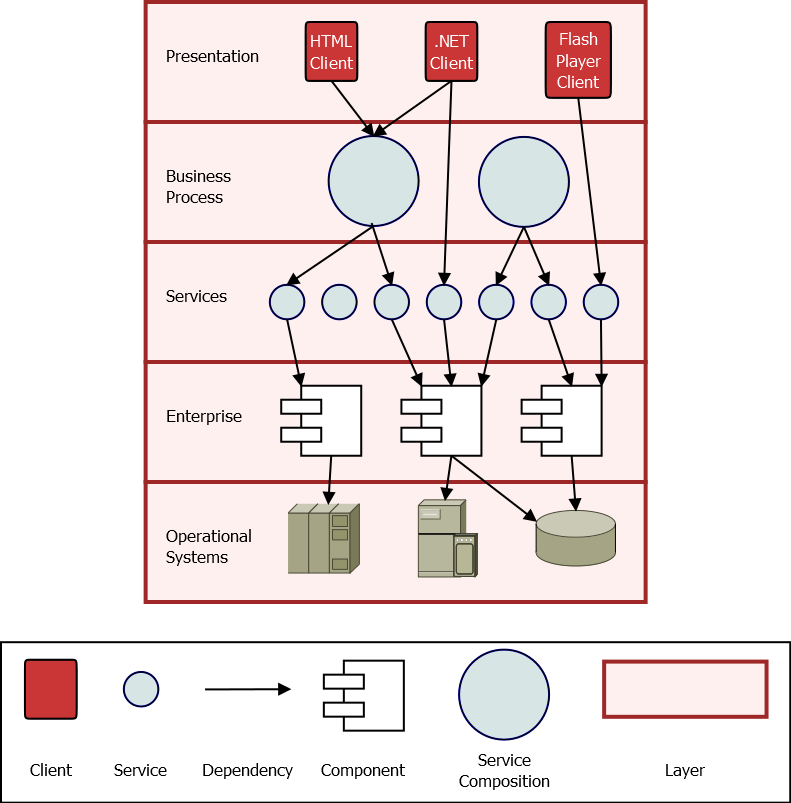
\includegraphics[scale=0.3]{Figures/SOA/SOA_layers.png}
  \end{center}
  \caption{Αρχιτεκτονικά επίπεδα ενός υπηρεσιοκεντρικού συστήματος}
  \label{fig:SOA_layers}
\end{figure}

\newcounter{numberedCntF}
\begin{enumerate}
\setcounter{enumi}{\thenumberedCntF}
\item \textbf{Business Process.} Οι υπηρεσίες που παρέχονται στο 
επίπεδο των υπηρεσιών, συνήθως συντίθενται σε ροές εργασίας (workflow) 
και βοηθούν στην ανάπτυξη εφαρμογών.
\item \textbf{Services.} Στο επίπεδο αυτό υπάρχουν οι υπηρεσίες. Η 
κλήση των υπηρεσιών καθορίζεται είτε κατά τη διάρκεια της σχεδίασης είτε 
μέσω μιας υπηρεσίας μητρώου (service registry) κατά τη διάρκεια 
εκτέλεσης.
\item \textbf{Enterprise.} Τα διάφορα κομμάτια που ανήκουν στο επίπεδο 
περιέχουν κώδικα που εξυπηρετεί τις ανάγκες των υπηρεσιών. Επίσης, 
παρέχεται πρόσβαση στα συστήματα που βρίσκονται στο κατώτερο επίπεδο.
\item \textbf{Operational Systems.} Εδώ ανήκουν όλα τα λειτουργικά 
εμπορικά και μη συστήματα.
\setcounter{numberedCntF}{\theenumi}
\end{enumerate}

Η δομική μονάδα του μοντέλου είναι η υπηρεσία. Η υπηρεσία είναι ένας 
μηχανισμός με τον οποίο επιτρέπεται πρόσβαση σε μια ή περισσότερες 
λειτουργίες. Η πρόσβαση παρέχεται μέσω μιας προκαθορισμένης διεπαφής και 
χρησιμοποιείται σύμφωνα με τους περιορισμούς και τις πολιτικές που 
ορίζονται από την περιγραφή της υπηρεσίας. Σύμφωνα με το αρχιτεκτονικό 
μοντέλο της OASIS \citep{OASIS-soa-raf} 
έχουμε διάφορους ρόλους σε μια υπηρεσία. Έχουμε 
αυτόν που προσφέρει την υπηρεσία και ονομάζεται Service Provider. 
Υπάρχει αυτός που ζητά την υπηρεσία για να την 
χρησιμοποιήσει/καταναλώσει και ονομάζεται Service Consumer. Έχουμε τον 
ρόλο του διαμεσολαβητή ο οποίος διευκολύνει την αλληλεπίδραση και τη 
συνδεσιμότητα στην προσφορά και χρήση της υπηρεσίας και ονομάζεται 
Service Mediator. Καταλήγοντας, έχουμε τον κάτοχο της υπηρεσίας ο οποίος 
ονομάζεται Service Owner.

Η κλήση μιας υπηρεσίας έχει το αποτέλεσμα είτε της επιστροφής 
πληροφορίας αν η αίτηση είχε τέτοιο σκοπό είτε της αλλαγής της 
κατάστασης του συστήματος. Σε καμία περίπτωση τον καταναλωτή της 
υπηρεσίας δεν τον ενδιαφέρει ο τρόπος παραγωγής της πληροφορίας ή πως 
έγινε η αλλαγή της κατάστασης. Επιπλέον, δεν γνωρίζει πώς υλοποιείται η 
υπηρεσία που χρησιμοποιεί. Παρακάτω αναφέρονται οι γενικές σχεδιαστικές 
αρχές που διέπουν μια υπηρεσία.

\subsection{Χαρακτηριστικά Υπηρεσιών}

Συνολικά έχουμε δυο κατηγορίες αρχών \citep{Duggan2012}. Η πρώτη 
περιλαμβάνει τις αρχές που αφορούν τα σχεδιαστικά χαρακτηριστικά των 
υπηρεσιών. Αυτά είναι:

\newcounter{numberedCntI}
\begin{enumerate}
\item Τυποποιημένη σύμβαση υπηρεσίας (service contract)
\item Επαναχρησιμοποίηση υπηρεσίας (Service reusability)
\item Αυτονομία υπηρεσίας (Service autonomy)
\item Υπηρεσία χωρίς κατάσταση (Service statelessness)
\item Δυνατότητα ανακάλυψης υπηρεσίας (Service discoverability)
\setcounter{numberedCntI}{\theenumi}
\end{enumerate}

Η δεύτερη κατηγορία περιλαμβάνει τις αρχές που ρυθμίζουν τον τρόπο με 
τον οποίο θα εφαρμοστούν οι παραπάνω αρχές. Αυτές είναι:

\newcounter{numberedCntJ}
\begin{enumerate}
\item Χαλαρή σύνδεση (Service loose coupling)
\item Αφαιρετικότητα (Service abstraction)
\item Δυνατότητα σύνθεσης (Service composability).
\setcounter{numberedCntJ}{\theenumi}
\end{enumerate}
Στη συνέχεια αναλύονται εκείνες οι αρχές που έχουν νόημα για το επίπεδο 
και το μέγεθος του συστήματος που χτίζουμε.

\subsubsection{Τυποποιημένη σύμβαση υπηρεσίας}

Είναι πολύ σημαντικό και αναγκαίο η ύπαρξη σαφών και καλώς 
ορισμένων συμβάσεων και διεπαφών που ενθυλακώνουν τα στοιχεία και τις 
λειτουργίες του συστήματος. Οι πόροι που προσφέρονται από μια υπηρεσία 
πρέπει να διαχειρίζονται μέσω αυτών των συμβάσεων. Δεν πρέπει δηλαδή να 
υπάρχει απευθείας σύνδεση των καταναλωτών της υπηρεσίας με τους 
υποκείμενους πόρους της. Η ανάγκη μας οδηγεί σε αυτή την αρχή είναι η 
χαλαρή συνδεσιμότητα μεταξύ της υπηρεσίας και του χρήστη της. 

Ο καταναλωτής της υπηρεσίας κατ' επέκταση δεσμεύεται από την σύμβαση 
αυτή προκειμένου να έχει πρόσβαση στην υπηρεσία. Η δέσμευση υπάρχει σε 
τέσσερα σημεία:

\newcounter{numberedCntBA}
\begin{enumerate}
\item Την περιγραφή των λειτουργιών που προφέρει η υπηρεσία.
\item Την περιγραφή του μοντέλου των δεδομένων που θα χρησιμοποιηθεί για 
την ανταλλαγή δεδομένων μεταξύ υπηρεσίας και χρήστη.
\item Θέματα που αφορούν την ποιότητα των παρεχόμενων υπηρεσιών (QoS)
\item Τον καθορισμό του τρόπου σύνδεσης του χρήστη με την υπηρεσία.
\setcounter{numberedCntBA}{\theenumi}
\end{enumerate}

\subsubsection{Επαναχρησιμοποίηση υπηρεσίας}

Το να είναι επαναχρησιμοποιήσιμη μια μονάδα λογισμικού είναι 
πολύ σημαντικό χαρακτηριστικό. Τα κατάλληλα επίπεδα αφαιρετικότητας 
βοηθούν στο να επιτευχθεί η αρχή αυτή.

\subsubsection{Αυτονομία υπηρεσίας}

Οι υπηρεσίες που προσφέρει το σύστημα πρέπει να είναι αυτόνομες 
μεταξύ τους. Η σχεδίαση αυτών πρέπει να γίνει με τέτοιο τρόπο ώστε να 
αποφευχθεί οποιαδήποτε επικάλυψη λειτουργικότητας μεταξύ τους. Επίσης, 
οι υπηρεσίες πρέπει να είναι αξιόπιστες ώστε να έχει νόημα η 
επαναχρησιμοποίηση τους. Για να επιτευχθεί αυτό η υπηρεσία έχει τον 
πλήρη έλεγχο στο πώς λειτουργεί. Εξωτερικοί-απομακρυσμένοι πόροι στους 
οποίους δεν υπάρχει έλεγχος δεν πρέπει να επηρεάζουν αρνητικά. 

\subsubsection{Υπηρεσία χωρίς κατάσταση}

Το να μην αποθηκεύεται κατάσταση σε μια υπηρεσία είναι θεμιτό 
αφού προωθεί την επαναχρησιμοποίηση της.

\subsubsection{Χαλαρή σύνδεση}

Τα κίνητρα πίσω από αυτήν την αρχή είναι η δυνατότητα 
επαναχρησιμοποίησης και συντήρησης. Ανεξάρτητες μονάδες λογισμικού 
καλύπτουν εύκολα αυτά τα χαρακτηριστικά. Όσο πιο σφιχτά συνδεδεμένα 
είναι τα στοιχεία του συστήματος όσον αφορά λειτουργικές εξαρτήσεις, 
τόσο περισσότερο αυξάνει η πιθανότητα να εξαπλωθεί και να επηρεάσει μια 
αλλαγή \citep{Meyer1994}. Το μειονέκτημα που εισάγεται όμως, είναι η 
προσθήκη επιπλέον επιπέδων αφαιρετικότητας με τις όποιες συνέπειες που 
έχει αυτό στην απόδοση του συστήματος.

\subsubsection{Αφαιρετικότητα}

Για να υλοποιηθεί σωστά η σύμβαση που προσφέρει η υπηρεσία, η 
σχεδίαση πρέπει να έχει τα απαραίτητα επίπεδα αφαιρετικότητας. 
Παράδειγμα, στη σύνδεση μεταξύ του παρόχου μιας υπηρεσίας και του 
καταναλωτή της διαμεσολαβεί η σύμβαση/διεπαφή αυτής. Αυτό έχει ως 
συνέπεια την απομόνωση εκείνου του κομματιού της υπηρεσίας, όπως είναι η 
υλοποίησή της, το οποίο δεν αποτελεί χρήσιμη γνώση στον χρήστη της. 

Υπάρχουν και άλλα σημεία στο σύστημα που επωφελούνται από αυτή 
την αρχή. Η πλατφόρμα, τα διάφορα πρωτόκολλα, τα δεδομένα και η δομή 
τους αποτελούν όλα διαφορετικά επίπεδα αφαρετικότητας.

\subsubsection{Δυνατότητα σύνθεσης}

Οι υπηρεσίες είναι σχεδιασμένες έτσι ώστε να μπορούν να 
συνδυαστούν και να προκύψουν διαδικασίες που έχουν νόημα για την 
εφαρμογή. Στα υπηρεσιοκετρικά συστήματα η σύνθεση μπορεί να επιτευχθεί 
με την ενορχήστρωσης όπου υπάρχει ένας καθοδηγητής που καθορίζει τον 
ρόλο της κάθε υπηρεσίας. Μπορεί να γίνει επίσης με την χορογραφία όπου 
κάθε υπηρεσία παίζει τον ρόλο της παράγοντας και εκδίδοντας γεγονότα που 
προκύπτουν κατά την εκτέλεσή της και λαμβάνει τα απαραίτητα γεγονότα για 
να επιτελέσει τον ρόλο της.
